\section{Theorie}
\label{sec:theorie}
Zunächst sollen die theoretischen Grundlagen für des Versuches erläutert werden.
Ausgehend von der Bandstruktur in Halbleitern werden Dotierung und schließlich der Faraday-Effekt behandelt.

% - effektive Masse
% - zirkulare Doppelbrechung
% - Faraday-Rotation / Faraday-Effekt

% - Bandstruktur
% - Dotierung
% - Faraday-Effekt

\subsection{Bandstruktur}
Die elektrischen Eigenschaften von kristallinen Festkörpern werden durch das Bändermodell beschrieben.
Aus dem periodischen Potential der Atomrümpfe entstehen im Kristall einzigartige Energieebenen,
die in \emph{Bänder} zusammengefasst werden und zusammen die \emph{Bandstruktur} bilden.
Es wird zwischen \emph{Leitungsband} und \emph{Valenzband} unterschieden.
    Im Valenzband befinden sich die Ladungsträger, die aufgrund ihrer geringeren Energie an den Atomkernen gebunden sind.
    Sie tragen daher nicht zur elektrischen Leitfähigkeit bei.
    %
    Im Leitungsband befinden sich hingegen die Ladungsträger,
    die aufgrund ihrer höheren Energie die Potentialtöpfe der Atomrümpfe überwinden können und frei beweglich sind.
    % Sie tragen zur elektrischen Leitfähigkeit bei.

Abhängig von dem Abstand zwischen Valenzband und Leitungsband – auch Bandlücke genannt – wird zwischen Isolatoren, Halbleitern und Leitern unterschieden.
    In Leitern verschwindet die Bandlücke und die Elektronen sind auf Valenzband und Leitungsband verteilt.
    %
    Bei Isolatoren ist die Bandlücke zu groß, um Elektronen aus dem Valenzband in das Leitungsband zu übertragen.
    Hier ist nur das Valenzband mit Elektronen besetzt.
    %
    Halbleiter liegen zwischen diesen beiden Extremen.
    Die Bandlücke ist klein genug, dass Elektronen durch Anregung aus dem Valenzband in das Leitungsband übertragen werden können.
    % Die Grenze zwischen Halbleitern und Isolatoren wird üblicherweise bei Bandlücken von $\SI{3}{\electronvolt}$ gezogen. [citation needed]


% \subsection{Effektive Masse}
Die Elektronen im Leitungsband eines Halbleiters sind nicht frei beweglich,
sondern werden durch das (nahezu) periodische Potential der Atomrümpfe gebremst.
Dieser Effekt lässt sich durch die Einführung einer \emph{effektiven Masse} $m^*$ beschreiben.
Aus einem Vergleich der Bewegungsgleichung im Kristall mit derjenigen im Vakuum ergibt sich
\begin{equation*}
    m^* = \hbar^2 \left. \frac{\mathrm{d} k^2}{\mathrm{d}^2 \epsilon} \right\rvert_{k=0}
    \; .
\end{equation*}


\subsection{Dotierung}
Durch Dotierung können die elektrischen Eigenschaften von Halbleitern verändert werden,
indem Fremdatome in das Gitter aus vier-wertigen Atomen eingefügt werden.
Im Fall von fünf-wertigen Atomen % beispielsweise \ce{XY}
bleibt jeweils ein Elektron übrig,
das nicht zur Bindung beiträgt und daher mit wenig Energie in das Leitungsband gehoben werden kann.
Das Fremdatom heißt dann \emph{Donator} und entsprechend der negativen Ladung im Leitungsband wird von \emph{n-Dotierung} gesprochen.
%
% ↓ für diesen Versuch nicht relevant
Bei \emph{p-dotierten} Halbleitern werden hingegen drei-wertige Fremdatome (\emph{Akzeptoren}) eingefügt,
deren fehlendes Bindungselektron leicht von anderen Atomen übernommen werden kann.
Diese Elektronenfehlstellen im Valenzband werden als \emph{Löcher} bezeichnet und verhalten sich wie positive Ladungsträger.
%
In beiden fällen sorgen die zusätzlichen freien Ladungsträger für eine starke Erhöhung der elektrischen Leitfähigkeit.
\autoref{fig:dotierung} stellt beide Dotierungstypen schematisch gegenüber.
Darin ist auch die Fermi-Energie $E_\text{F}$ angegeben.

\begin{figure}
    \centering
    \begin{subfigure}{0.48\textwidth}
        \centering
        \includegraphics[width=\textwidth]{content/img/Demtröder_14.13.pdf}
        \caption{n-dotiert}
        \label{fig:dotierung:donatoren}
    \end{subfigure}
    \hfill
    \begin{subfigure}{0.48\textwidth}
        \centering
        \includegraphics[width=\textwidth]{content/img/Demtröder_14.14.pdf}
        \caption{p-dotiert}
        \label{fig:dotierung:akzeptoren}
    \end{subfigure}
    \caption{Energieschemata unterschiedlich dotierter Halbleiter \cite{demtroeder}.}
    \label{fig:dotierung}
\end{figure}


\subsection{Faraday-Effekt}
% \emph{Zirkulare Doppelbrechung} beschreibt die Fähigkeit eines Kristalls,
% die Polarisationsebene eines linear polarisierten Lichtstrahls bei der Transmission zu drehen \cite{anhang}.
%
Es wird eine elektromagnetische Welle betrachtet, die sich in z-Richtung ausbreitet.
Sie kann in einen rechts- und einen links-zirkular polarisierten Anteil zerlegt werden:
\begin{equation*}
    % Quelle: Anhang zur Versuchsanleitung
    E(z) = \frac{E_\text{R}(z) + E_\text{L}(z)}{2} \; .
\end{equation*}
Wenn die Phasengeschwindigkeit der beiden Anteile unterschiedlich ist,
wird die Polarisationsebene linear polarisierten Lichts beim Durchgang durch den Halbleiter gedreht,
    wie in \autoref{fig:zirkulare_doppelbrechung} dargestellt.
Allgemein wird dieses Phänomen als \emph{zirkulare Doppelbrechung} bezeichnet.
Für den Drehwinkel $\theta$ gilt
\begin{equation*}
    \theta
    = \frac{L}{2}(k_\text{R} - k_\text{L})
    = \frac{L \omega}{2} \left(
        \frac{1}{v_\text{Ph,R}} -
        \frac{1}{v_\text{Ph,L}}
    \right)
    = \frac{L \omega}{2 c} (n_\text{R} - n_\text{L}) \; ,
\end{equation*}
wobei
    $L$ die Weglänge im Material,
    % $k_\text{L/R}$ …
    $\omega$ die Wellenfrequenz,
    % $v_\text{Ph,L/R}$ …
    $c$ die Lichtgeschwindigkeit im Vakuum
    und $n_\text{L/R}$ die Brechungsindizes
sind
und die Beziehungen
\begin{align*}
    % v_\text{Ph} &= \frac{\omega}{k}
    % \Leftrightarrow
    k &= \frac{\omega}{v_\text{Ph}}
    % &&\text{ und }&&
    &
    n &= \frac{c}{v_\text{Ph}}
\end{align*}
eingesetzt wurden.

Gewöhnlich tritt zirkulare Doppelbrechung nur bei optisch aktiver Materie auf.
Durch den Einfluss eines äußeren Magnetfeldes $\vec B$,
    das parallel zur Ausbreitungsrichtung der Lichtwelle verläuft,
kann das Phänomen jedoch auch bei optisch inaktiver Materie beobachtet werden,
was als \emph{Faraday-Effekt} oder \emph{Faraday-Rotation} bezeichnet wird.

Die Bewegungsgleichung
\begin{equation*}
    % Quelle: Anhang zur Versuchsanleitung (Gleichung 22)
    m \frac{\mathrm{d}^2 \vec r}{\mathrm{d} t^2} + K \vec r
    = - e_0 \vec E(\vec r) - e_0 \frac{\mathrm{d} \vec r}{\mathrm{d} t} \times \vec B
\end{equation*}
beschreibt die Wechselwirkung eines gebundenen Elektrons mit dem äußeren Magnetfeld $\vec B$ und dem elektrischen Feld $\vec E$ der Lichtwelle.
Dabei sind
    $\vec r$ die Auslenkung aus der Ruhelage,
    $K$ eine Konstante für die Kopplung an die Umgebung des Elektrons
    und $e_0$ die Elementarladung.
Der Einfluss des magnetischen Felds der Lichtwelle kann hier vernachlässigt werden.
%
    Für eine ebene Welle $E(t) \propto \exp(-i \omega t)$
    und mit der makroskopischen Polarisation $\vec P = -N e_0 \vec r$
ergibt sich aus der vorherigen Gleichung
\begin{equation*}
    % Quelle: Anhang zur Versuchsanleitung (Gleichung 23)
    -m \omega^2 \vec P + K \vec P
    = + e_0^2 N \vec E + i e_0 \omega \vec P \times \vec B
\end{equation*}
mit der Anzahl $N$ der Elektronen pro Einheitsvolumen.

% NOTE: Ich gebe hier nur einen Überblick über die Herleitung. Alles andere würde den Rahmen sprengen.
Für ein äußeres Magnetfeld in $z$-Richtung wird
    über den Zusammenhang $\vec P = \epsilon_0 \chi \vec E$
der dielektrische Suszeptibilitäts-Tensor $\chi$ eingeführt.
$\epsilon_0$ ist dabei die Permittivität des Vakuums.
Bei Betrachtung der Komponente $\chi_{xy}$ zeigt sich,
dass diese
    imaginär
    und konjugiert komplex zu der anderen Nebendiagonalkomponente $\chi_{yx}$
ist,
was gerade Doppelbrechung impliziert.
Der vollständige Tensor $\chi$ hat die Form
\begin{equation*}
    \chi = \begin{pmatrix}
        % Warum auch immer das i nicht in den Komponenten enthalten ist…
        % Aber im Anhang steht es eben so.
        \phantom{i}\chi_{xx} & i\chi_{xy} & 0 \\
        i\chi_{yx} & \phantom{i}\chi_{yy} & 0 \\
        0 & 0 & \chi_{zz}
    \end{pmatrix} \; .
\end{equation*}

Nach
    einer Betrachtung der Frequenzabhängigkeit
        (die Resonanzfrequenz $\omega_0$ wird als hinreichend verschieden von der Messfrequenz $\omega$ angenommen)
    und dem Übergang von $m$ zur effektiven Masse $m^*$
lautet schließlich
die (von der Weglänge unabhängige) Faraday-Rotation pro Einheitslänge
\begin{equation}
    % Quelle: Anhang zur Versuchsanleitung
    \theta_\text{frei}
    = \frac{\theta}{L}
    = \frac{e_0^3}{8 \pi^2 \epsilon_0 c^3} \frac{1}{{m^*}^2} \lambda^2 \frac{N B}{n} \; .
    \label{eqn:theta_frei}
\end{equation}


\begin{figure}
    \centering
    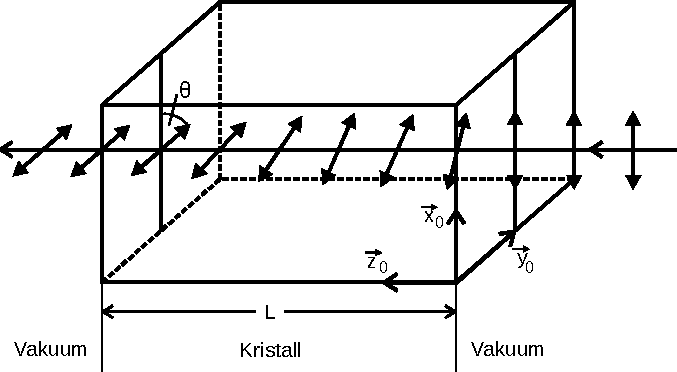
\includegraphics[width=0.75\textwidth]{content/img/Anhang_Abb_1.pdf}
    \caption{Drehung der Polarisationsebene einer Lichtwelle beim Durchgang durch einen Halbleiter \cite{anhang}.}
    \label{fig:zirkulare_doppelbrechung}
\end{figure}
